\documentclass[acmtog]{acmart}
% Title portion
\title{Tetrahedralization and Volume Rendering (B)} 
\author{Name:\quad Ziyi Yu, Chuan Li, Yuhang Gong   \\ student number:\quad 2018533124, 2018533234, 2018533180
	\\email:\quad yuzy, licha, gongyh}
%\author{Name: Chuan Li   \\ student number:\quad 2018533234
%	\\email:\quad licha@shanghaitech.edu.cn}
%\author{Name: Yuhang Gong  \\ student number:\quad 2018533180
%	\\email:\quad gongyh@shanghaitech.edu.cn}


% Document starts
\begin{document}
\maketitle

\vspace*{2 ex}

% INTRODUCTIONNNNNNNNNNNN
\section{Introduction}
Volume visualization is useful in many areas. We focus on directly rendering unstructured tetrahedral meshed where volume's interior needs to be visualized. There are many approaches to rendering unstructured grids and accuracy is usually important. Ray-casting-based methods, which our work focuses on, are widely accepted.\\
Tetrahedralization means to collect data into multiple tetrahedrons, while some datasets have already implemented this process. Tetrahedralized volume rendering has a better usage of input data and a more efficient calculation especially in the transparent area. Whereas its intuition and procedure are very much familiar to the former one's. 

% IMPLEMENTATION DETAIL
\section{Implementation Details}
% 11111111111111111111 Tetrahedralization
\subsection{Tetrahedralization}
\begin{figure}[h]
\centering
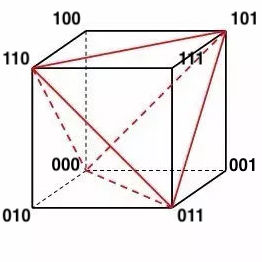
\includegraphics[height=5cm]{figure/cube.jpg}
\caption{5 Tetrahedra within a Cube}
\end{figure}
In homework 5, cubes are used as the voxels to apply interpolation, 
each non-boundary vertex, oriented at the origin, with its adjacent seven vertices compose a cube voxel. Rather in this project, tetrahedrons are used as the voxels to perform volume rendering.
\\One practical way to complete the task is to divide each existed cube into five tetrahedrons.
Taking each non-boundary vertex as the origin, labeled as 000, and connecting diagonals in all six faces will produce five tetrahedrons within a cube. The five tetrahedra vertex sets can be labeled as
\{000, 001, 011, 101\}, \{000, 011, 010, 110\}, \{000, 100, 110, 101\}, \{000, 110, 011, 101\}, \{111, 101, 110, 011\}.

% 2222222222222222222 SSC
\subsection{Compute Screen Space Projection Coordinates}
\begin{figure}[h]
\centering
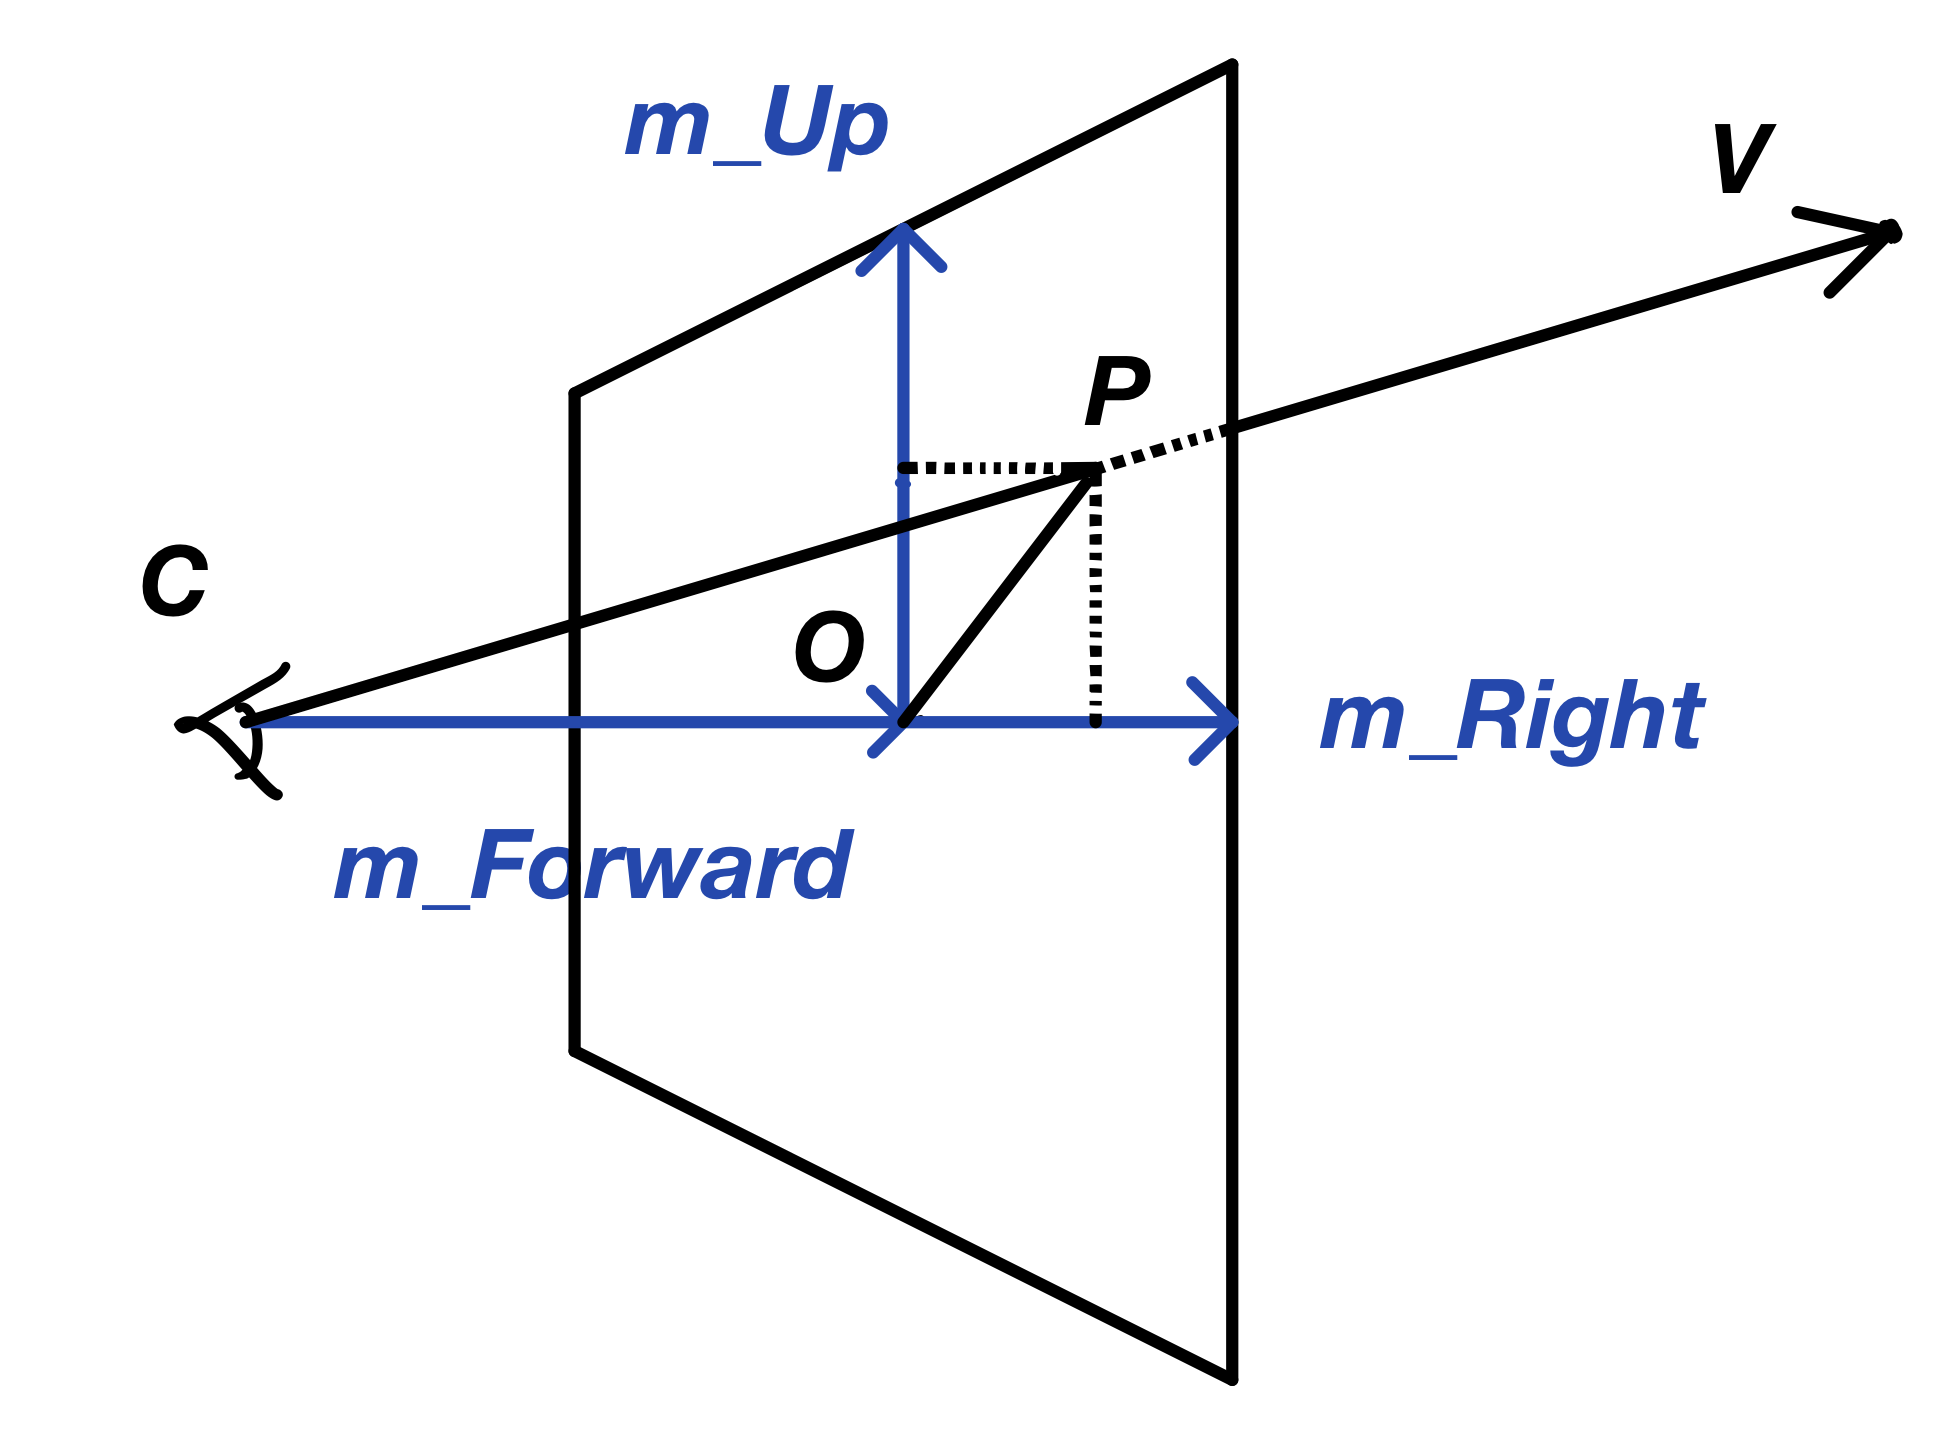
\includegraphics[height=5cm]{figure/NbSSC}
\caption{Screen Space Projection}
\end{figure}
In this stage, we calculate every vertex’s screen space coordinate (SSC) in order to tell which tetrahedron(s) cover a single claimed pixel. Firstly we have known that \emph {Camera} has a unit vector 
\textbf{m\_Forward} 
(\textbf{CO} in Fig. 2) pointing at the center of film, two vectors \textbf{m\_Right} and \textbf{m\_Up} as the graph shows with magnitude of half of physical length and width of the film. Given a vertex \textbf{V} in the view, we have its screen projection \textbf{P} with 
\begin{equation} 
\boldsymbol {CP} = t \cdot
\boldsymbol{CV}
\quad (0<t<1)
\end{equation} 
Derive \emph{t} by solving 
\begin{equation} 
\boldsymbol {CO}\cdot \boldsymbol{OP}=0
\end{equation} since \textbf{m\_Forward} is always orthogonal to the screen by initial construction. Then we calculate \textbf{OP}’s projection on \textbf{m\_Right} and \textbf{m\_Up} to obtain its coordinate, and subsequently the coordinate with respect to pixel (e.g. lower left corner’s pixel point (0,0), up right corner’s pixel point (1023,1023)). 

% 333333333333333333333 Extract
\subsection{Extract Intersection Records}
The screen space projection of tetrahedra is implemented in this step. Since screen space projection of vertices have already been calculated and stored in SSC, we can directly access the projected 2D coordinates of the 4 vertices of a tetrahedron via vertex index. By inspection, the projected shape of a tetrahedron can be either a quadrilateral or a triangle(a concave quadrilateral).
\\The purpose of screen space projection of tetrahedra is to find out all tetrahedra a ray shooting from a specific pixel intersected with. Every pixel covered by the projected shape of a tetrahedron is considered affected by this tetrahedron in pixel color.
\\
Before we project tetrahedra, a few helper functions are need to simplify our processing.
\subsubsection{Helper function: cross product}
Cross product function basically takes in 2 2D vectors 
\textbf {vA},\textbf {vB}, then return a scalar
\begin{equation} 
\boldsymbol {vA}.x \cdot 
\boldsymbol {vB}.y - 
\boldsymbol {vB}.x \cdot 
\boldsymbol {vA}.y
\end{equation} 

This function is important and have been used a lot in following parts. 

\subsubsection{Helper function: the side of line}
Given a line shooting from point \emph{pA} to point \emph{pB}, we need to decide whether point \emph{pC} is above the line or below the line. This is achieved by cross product $\overrightarrow{CA}$ and $\overrightarrow{AB}$. If the result > 0, then \emph{pC} is above the line; if the result = 0, \emph{pC} is on the line; if the result < 0, \emph{pC} is below the line.

\subsubsection{Helper function: point inside triangle}
We need to decide whether a point \emph{pP} is inside a triangle connected by \emph{pA}, \emph{pB} and \emph{pC}. This is easily achieved by justifying \emph{pP} and \emph{pA} are on the same side of $\overrightarrow{pBpC}$, \emph{pP} and \emph{pB} are on the same side of $\overrightarrow{pApC}$, \emph{pP} and \emph{pC} are on the same side of $\overrightarrow{pApB}$.

\subsubsection{Case1: the projection is a triangle}
\begin{figure}[h]
\centering
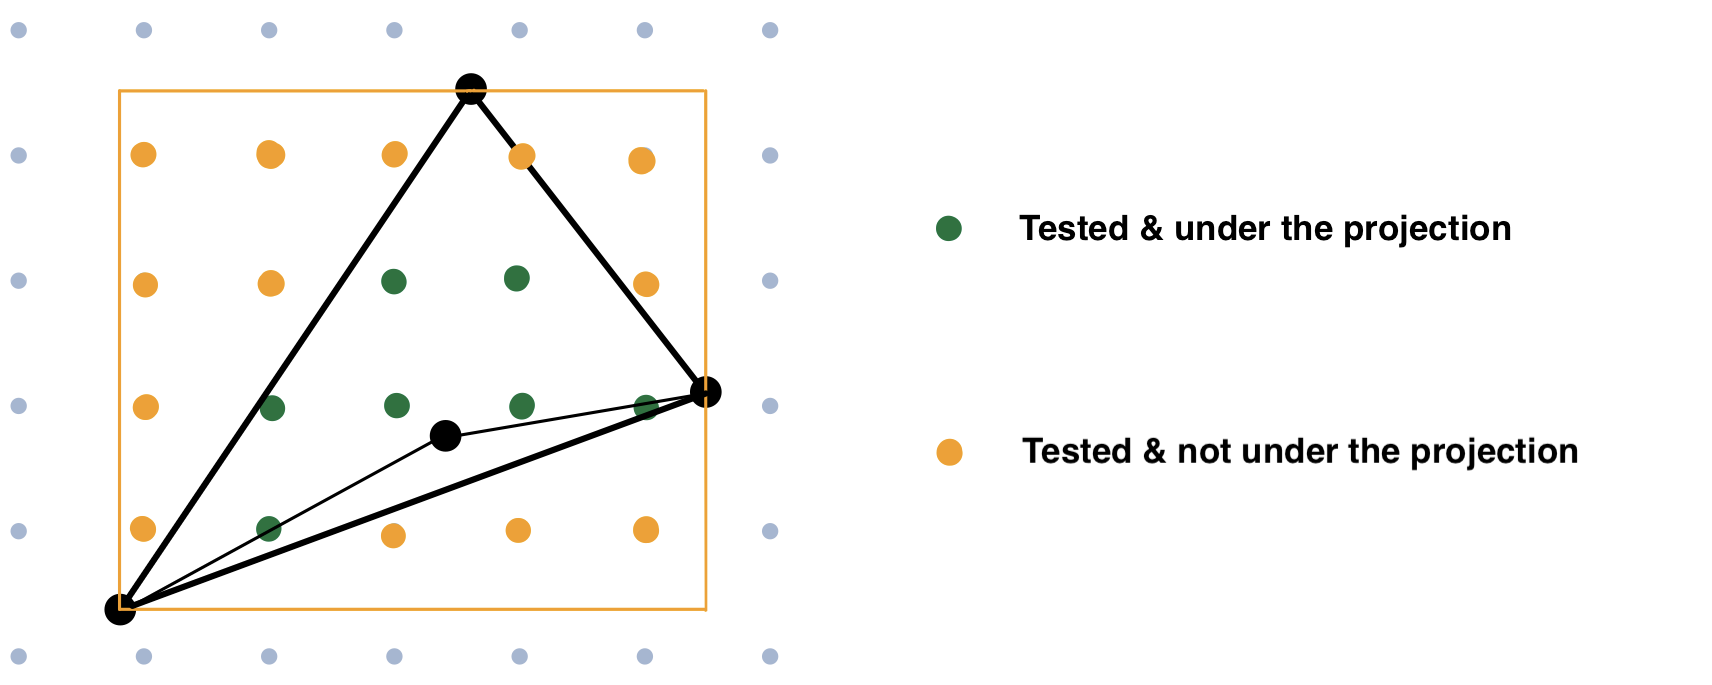
\includegraphics[height=3.7cm]{figure/triangle}
\caption{Triangular Projection}
\end{figure}
By testing whether there exists one of the four projected vertices of a tetrahedra inside the triangle formed by the rest of 3 vertices, we can easily find out whether the projection is a triangle or a quadrilateral.
\\If the projection is a triangle, we can easily decide what pixels are inside this triangle and then push this tetrahedron to the \textbf{PerPixelIntersectionList}.
\\To narrow the range of pixels to be decided, we only test pixels inside a square ranging from the minimum of x,y coordinates of the four vertices to the maximum of x,y coordinates.

\subsubsection{Case2: the projection is a quadrilateral}
\begin{figure}[h]
\centering
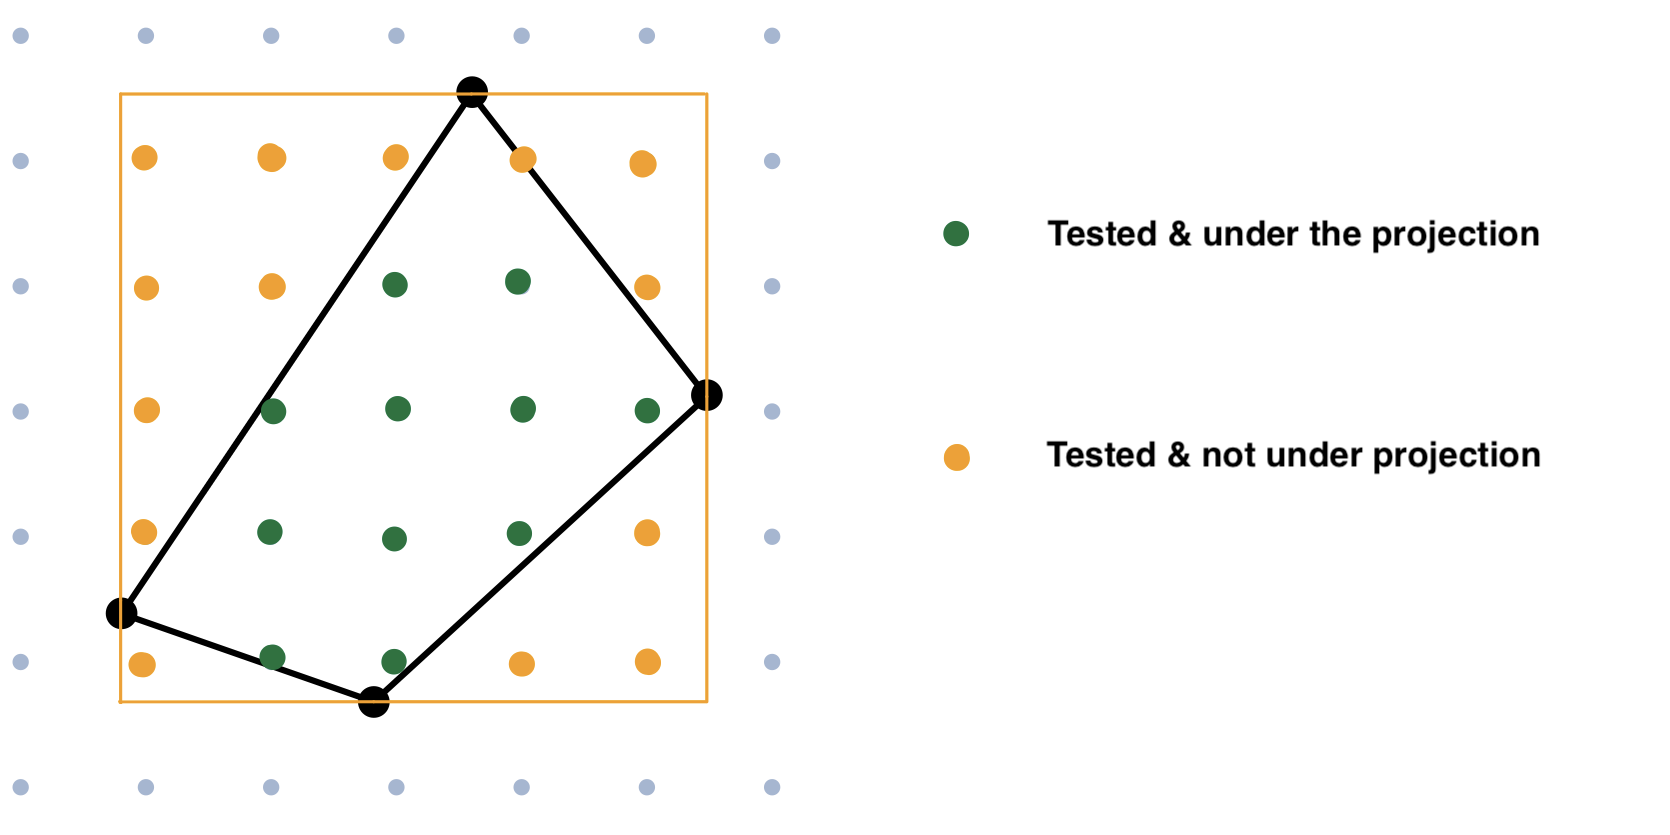
\includegraphics[height=4cm]{figure/quadri}
\caption{Quadrilateral Projection}
\end{figure}
If the projection is a quadrilateral, the deciding process is a little bit complex. First of all, we need to find the correct connecting order of the 4 vertices clockwise. This can be achieved by finding out the leftmost and rightmost points \emph{pL}, \emph{pR}, then do $\overrightarrow{pLpR}$ line\_side test for the rest 2 vertices.
\\Now that we have \emph{pA},\emph{pB},\emph{pC},\emph{pD} 4 vertices clockwise, a popular method to decide whether pixel \emph{pP} is inside the quadrilateral is to do cross product $\overrightarrow{pApB}$ and $\overrightarrow{pApP}$, $\overrightarrow{pBpC}$ and $\overrightarrow{pBpP}$, $\overrightarrow{pCpD}$ and $\overrightarrow{pCpP}$, $\overrightarrow{pDpA}$ and $\overrightarrow{pDpP}$ separately, and test whether the second vector is on the clock wise direction of the first vector. If all of the above conditions are true, then \emph{pP} is inside quadrilateral \textbf{pApBpCpD}. Push this tetrahedron to \textbf{PerPixelIntersectionList}.

% 44444444444444444 Compute Effect
\subsection{Compute Intersection Effect}
\begin{figure}[h]
\centering
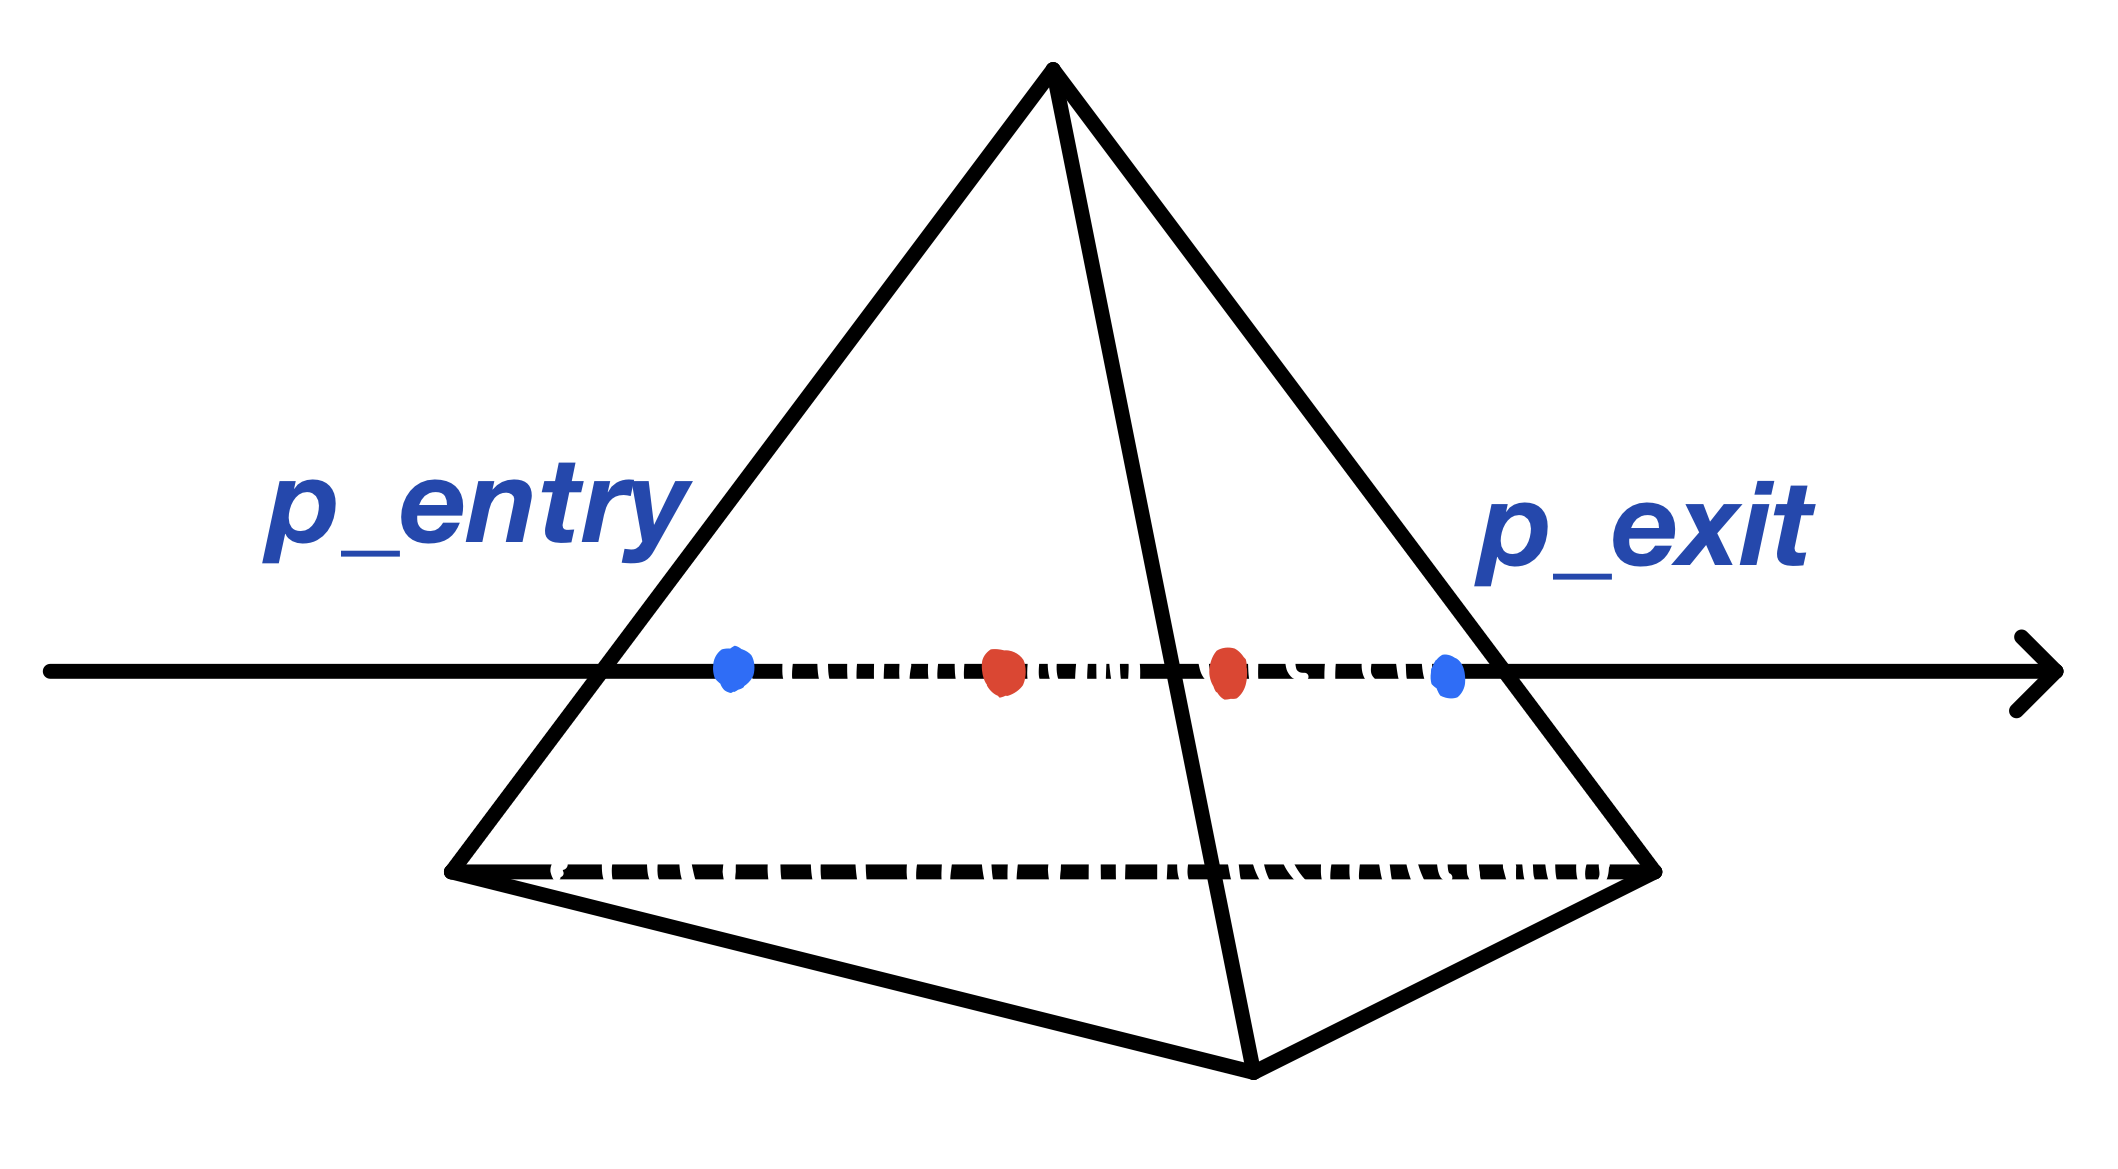
\includegraphics[height=4cm]{figure/NBCIE}
\caption{Calculate Intersection Effect}
\end{figure}
\subsubsection{Basic idea} 
We have known which tetrahedron(s) every pixel cover now. Suppose that the ray $R_{i,j}$ from camera to pixel(i,j) shoots through tetrahedrons a, b and c, we need to calculate 3 intersection effects: R with a, R with b, R with c individually. The first step calculates 2 intersection points (\textbf{p\_entry} and \textbf{p\_exit}) of the ray and one of the tetrahedrons being shot.\footnote{Due to the accuracy difference among various algorithms, the ray might miss some tetrahedrons even though they've covered the corresponding pixel in the third step.}
The distance between camera and \textbf{p\_entry} is recorded for the sorting phase. The ray’s path is divided into a predefined number (\emph{NumOfSamples}+1) of line segments. Iterating from \textbf{p\_entry}, the density of this point is interpolated using the 4 vertices of the tetrahedron. The color is determined by color map function. 
\\
As the ray travels from \textbf{p\_entry} to \textbf{p\_exit}, the color and intensity contributions can be approximated. The ray starts traveling with full intensity and each segment is assumed to have a uniform color, which is the color of \textbf{p\_entry}. The color contributions of the line segments to the pixel are proportional to the color attributes of the traveled region, the travel distance, the opacity coefficient of the region and the intensity of the ray itself. The ray loses most of its energy while traveling through nontransparent regions; thus later regions have a smaller effect on the final color. After the ray travels through all regions, its final color is recorded.
\subsubsection{Interpolation}
Accurately calculating the density of a point in or on a tetrahedron is important because poor interpolations may cause significant artifacts. The interpolation process starts by selecting a reference vertex, which can be any one of the tetrahedron’s vertices. Then we have $\boldsymbol{M}$ matrix which contains the coordinates of the other three vertices. The $\boldsymbol{N}$ vector stores the relative position of the input point to the reference vertex. The density vector $\boldsymbol{D}$ contains density differences of the vertices relative to the density of the reference vertices. Then the equation $\boldsymbol{M} \times \boldsymbol{R}=\boldsymbol{D}$ is solved to obtain $\boldsymbol{R}$ vector, which represents a coefficient vector that will give the relative density of a point when multiplied with the relative position vector of that point. Hence $\boldsymbol{R} \cdot \boldsymbol{N} + d_0$ is the final interpolated density of input point, where $d_0$ stands for the density of reference vertex. 
%555555555555555555555555 Sort
\subsection{Sort Intersection Effect List in Ascending Order by Distance}
We have calculated the intersection effect of a tetrahedron for the specific pixel. Since the composition step composites all tetrahedron effects from the nearest to the farthest (similar to rendering from front to back in our assignment), we sort the \textbf{IntersectionEffect} list in ascending order by its distance. This is achieved by the sort function from the standard library.

% 666666666666666666666666 Composition
\subsection{Composition}
To composite, for each pixel, we iterate its already sorted intersection effect list.
For each intersection, we update the destination color and opacity as the following equations:
\begin{gather} 
C_{color} = C_{color} + (1 - C_{opacity}) \cdot R_{color}\\
C_{opacity} = C_{opacity} + (1 - C_{opacity}) \cdot R_{opacity}
\end{gather}

Note that when the opacity is too high, we break the loop and stop composition.

\section{Results}
\begin{figure}
\begin{minipage}{0.48\linewidth}
	\centerline{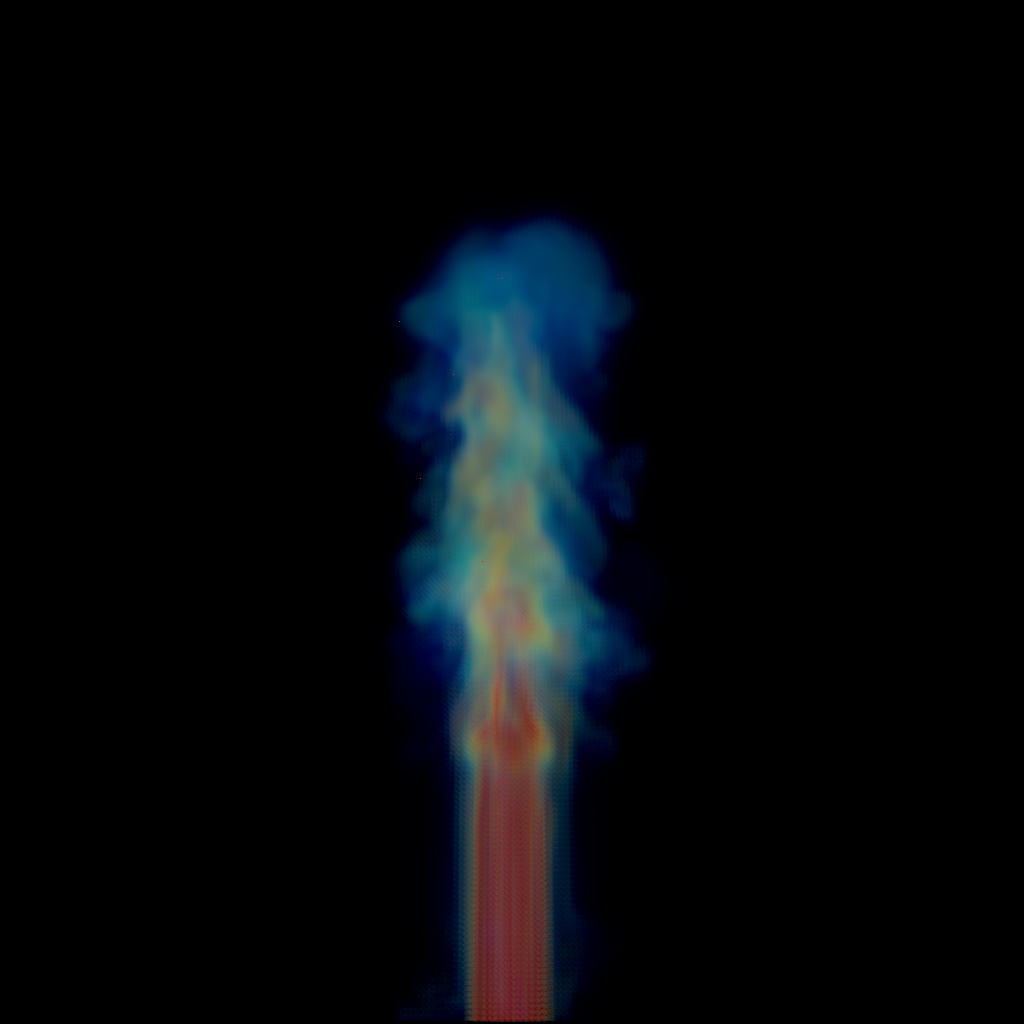
\includegraphics[width=4cm]{figure/tetra_vol_1sample}}
	\centerline{(a) Result 1}
\end{minipage}
\hfill
\begin{minipage}{0.48\linewidth}
	\centerline{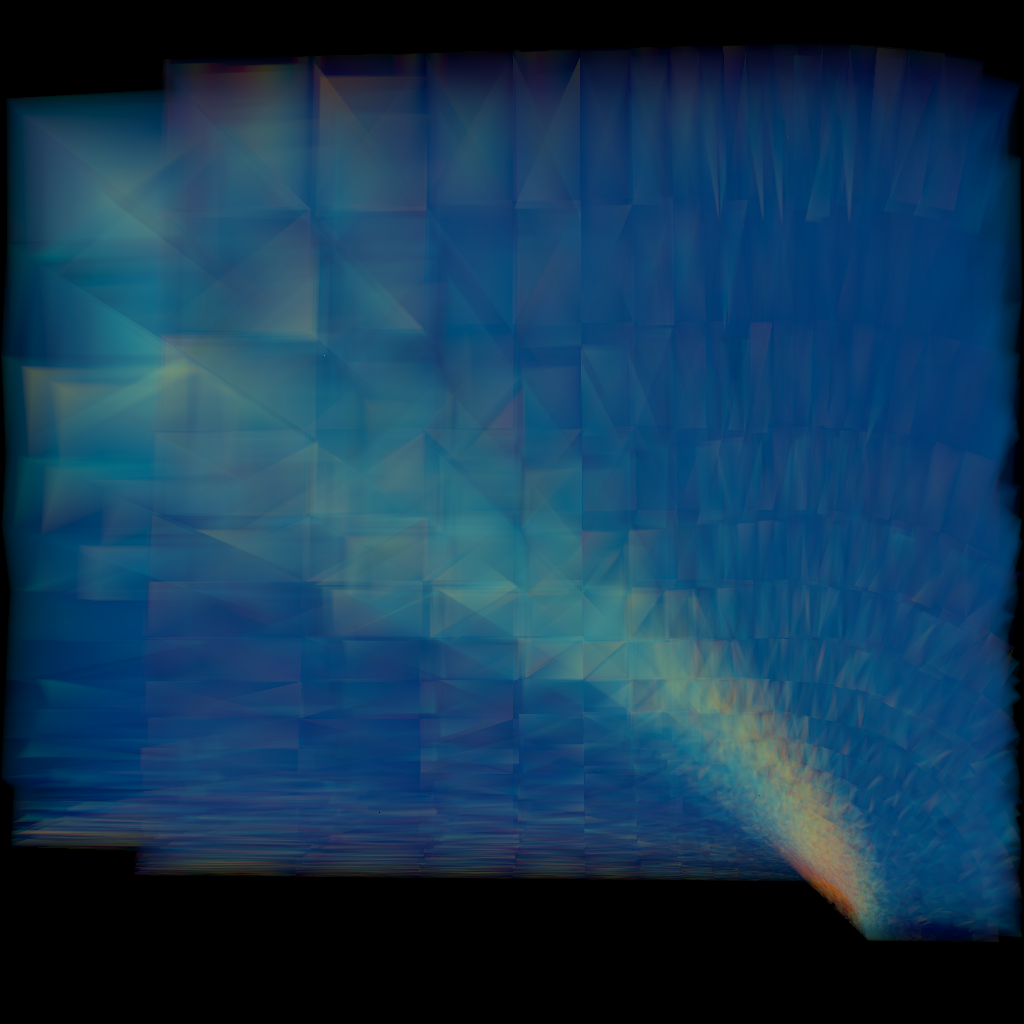
\includegraphics[width=4cm]{figure/blunt06jet}}
	\centerline{(b) Result 2}
\end{minipage}
\vfill
\begin{minipage}{0.48\linewidth}
	\centerline{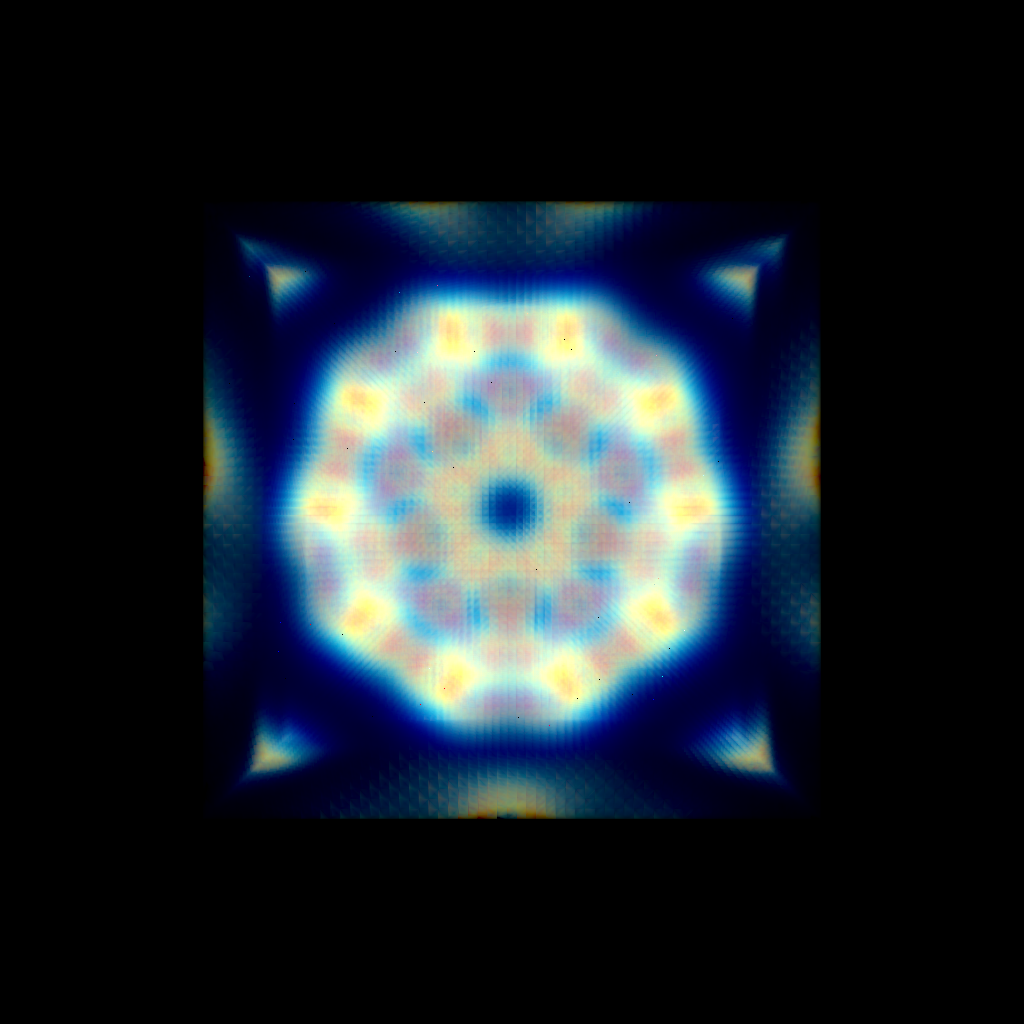
\includegraphics[width=4cm]{figure/bucky_jet}}
	\centerline{(c) Result 3}
\end{minipage}
\hfill
\begin{minipage}{0.48\linewidth}
	\centerline{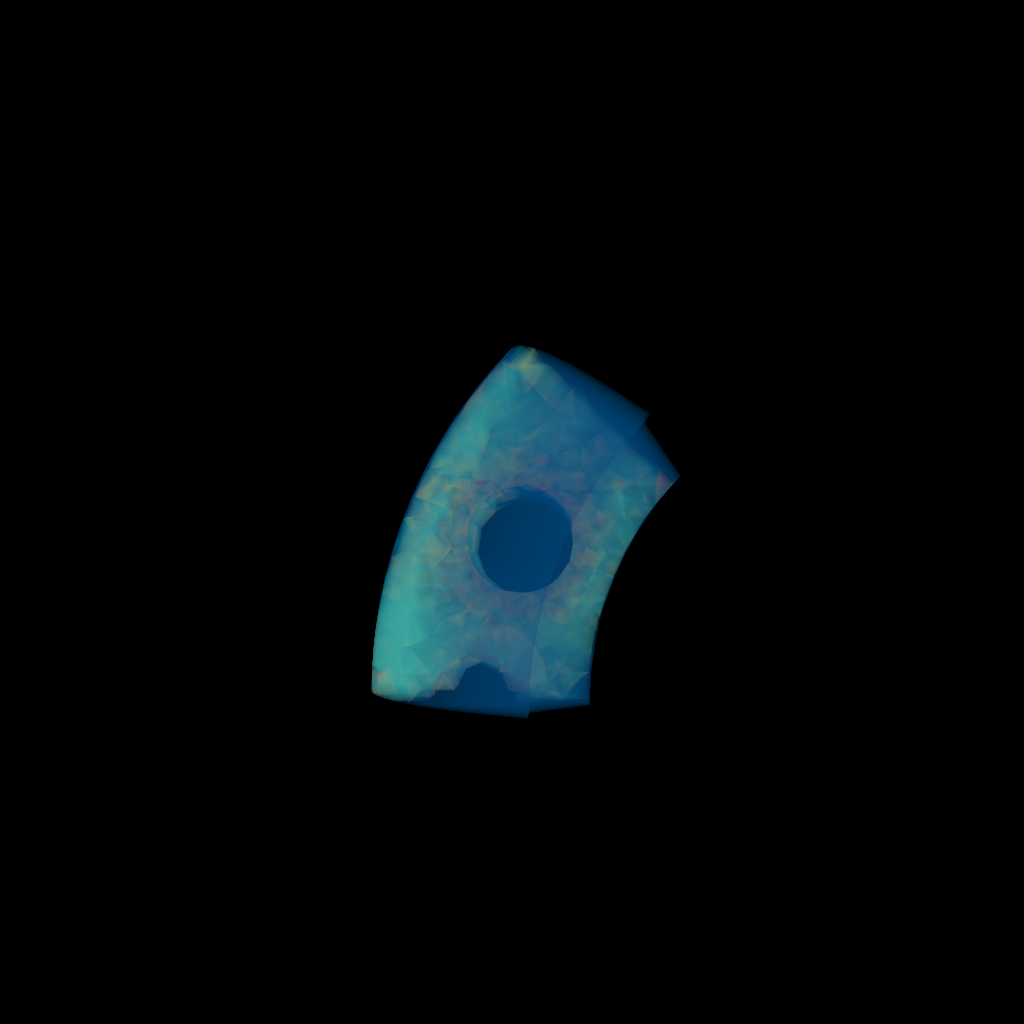
\includegraphics[width=4cm]{figure/spx_005_jet}}
	\centerline{(d) Result 4}
\end{minipage}
\caption{Rendering Results of 4 Datasets.}
\end{figure}





\end{document}
